\section{\system: Transformer for Timeseries}
\label{sec.rita}
In this section, we first introduce the overall \system approach. We then show how to use \system to support various downstream tasks. 

%Our goal is to develop a tool for general time series analytics tasks, not limited in generative task like time series prediction. With the feature extracted by Encoder, we can do classification/clustering on the global feature of time series; and do prediction/imputation/outliner detection on the local feature of target parts of time series.
\begin{sloppypar}

\subsection{The \system Encoder}
\label{sec.rita.encoder}

\subsubsection{The Overview\nopunct}\ \\
\noindent\textbf{The Key Idea.} \system leverages the Transformer Encoder~\cite{DBLP:conf/nips/VaswaniSPUJGKP17}. The Decoder in the Transformer is not used, because it is for generative tasks solely such as translation in NLP. In particular, each input sample of Transformer Encoder $\mathbf{X} \in \mathbb{R}^{n*d}$ represents the embeddings of $n$ semantic units (i.e. $n$ word embedding in NLP). Each embedding has $d$ dimensions. Then Encoder models the correlations between these semantic units and outputs $\mathbf{Y} \in \mathbb{R}^{n*d}$ as the context-aware embedding of these $n$ semantic units.

To fill the gap between timeseries and natural language, \system uses a {\bf time-aware convolution} strategy which chunks one input timeseries into $n$ windows and automatically produces one embedding per window. These embeddings are then fed into the Transformer Encoder as its input, as shown in Fig.~\ref{fig.convolution}.
The intuition is that timeseries are typically composed of a set of local patterns which have independent meanings and hence can be treated as the semantic units like words in natural language. For example, these patterns might represent cyber-security breaches, occurrences of seizures, or selling or buying opportunities in stock market.  

Inspired by the success of CNNs in computer vision tasks, which use {\it convolution} to capture the local structures in each image patch, we leverage convolution to capture the local patterns in timeseries. Treating a multi-channel timeseries as a matrix where each row represents one channel and each column corresponds to one timestamp and conducting a convolution operation on it, \system automatically discovers the correlations across different channels, thus naturally solving the multi-channel problem.


\begin{figure}[t]
%\vspace{-3mm}
    \centering
    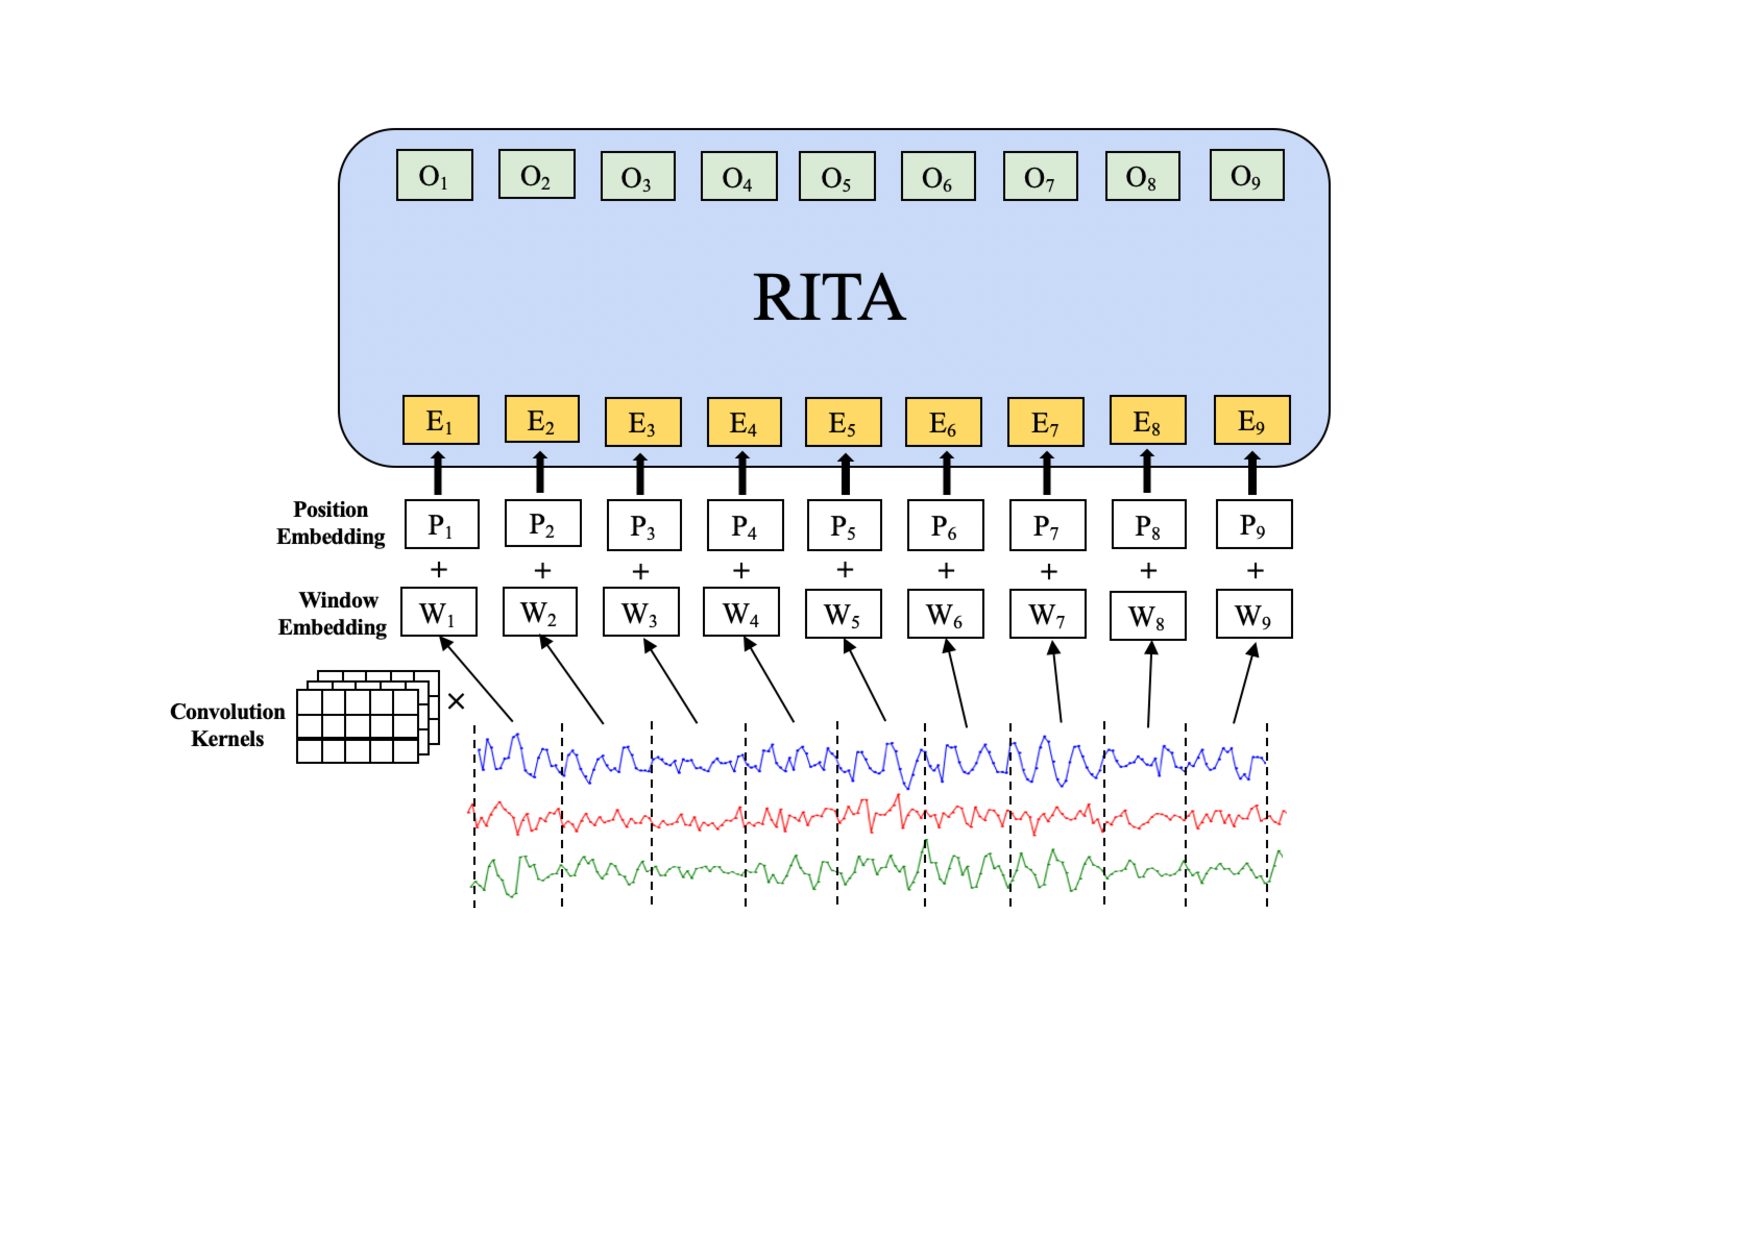
\includegraphics[width=1.0\columnwidth]{figures/rita_conv.pdf}
    \vspace{-5mm}
    \caption{Convolution in \system}
    \label{fig.convolution}
    \vspace{-6mm}
\end{figure}

\subsubsection{Technical Details\nopunct}\ \\
%\vspace{-1mm}
\noindent\textbf{Input Embedding.}
We denote a raw timeseries as $T \in \mathbb{R}^{t*m}$, which corresponds to a multi-channel (multivariate) timeseries of length $t$ with $m$ channels (variables). The input embedding $X$ to Transformer Encoder is generated by:
\vspace{-1mm}
\begin{equation}
\label{eq.convolution}
X_{i,j}=\sum_{k=0}^m  \sum_{l=0}^{KernelSize}W_{j,k,l}*T_{i+l,k}+ B_{j,k} 
\end{equation}

%\lei{Introduce in more details how convolution works. For example, what is a convolution kernel? what does d, m, kernelSize stand for? Convolution kernel is learned jointly with the transformer encoder, etc. Ideally, explain it with an example here. }

In Eq.~\ref{eq.convolution}, $B \in \mathbb{R}^{d*m}$ is bias. $W$ $\in$ $\mathbb{R}^{d \times m \times KernelSize}$ corresponds to the weight of the convolution layer, where $d$ represents the number of the convolution kernels and $m \times KernelSize$ defines one convolution kernel as a $m \times KernelSize$ matrix. The convolution kernel has $m$ rows, each corresponding to one channel of the timeseries. KernelSize defines the number of timestamps that each convolution kernel covers, identical to the window size in sliding window.  

The convolution kernel slides from left to right on the timeseries matrix over the time axis and computes the dot product with the corresponding timeseries sub-matrix covered by each window. In this way it produces one value for each window;  this value is the feature of this window. 
Because the convolution layer uses $d$ convolution kernels, it produces a $d$-dimensional feature embedding for each window. In Eq.~\ref{eq.convolution}, $X_{i,j}$ stands for the $j$th dimension of the embedding produced for the $i^{th}$ window.
Note the convolution kernels are learned jointly with the Transformer encoder. 

\noindent\textbf{Position Embeddings.}
As mentioned before, temporal order is important in timeseries analytics. We thus use position embedding to make \system aware of the time ordering among the local embeddings extracted by convolution. 
In addition, a special embedding vector \textbf{[CLS]} is attached at the start of input, serving as a global information aggregator.  
To be specific, input $Z$ is generated by $\mathit{Z=[CLS] \textcircled{+} (X+P)}$, where $\mathit{P=[p_1,p_2,...,p_n]}$, $p_i$ $\in$ $\mathbb{R}^d$ is the embedding of position $i$ and \textcircled{+} denotes concatenation. 
As is widely adopted in NLP, we use learnable position embedding~\cite{DBLP:conf/naacl/DevlinCLT19}, which means all $p_i$ are trainable parameters. 
%%try batch norm

\subsection{Downstream Tasks}
\label{sec.transformer.downstream}

The \system Encoder supports a variety of downstream tasks, as shown in Fig.~\ref{fig.overview}. In this section, we show that with minimal modification \system encoder is able to effectively support classification, imputation and forecasting tasks. 
Other unsupervised analytics tasks such as similarity search or clustering are naturally supported by extracting feature embeddings from \system encoder.

\subsubsection{Classification\nopunct}\ \\
Timeseries classification is of great importance in many real-world applications, such as human activity recognition(HAR) and disease diagnosis on electrocardiogram data.

To classify timeseries, we input timeseries to the model as described in Sec.~\ref{sec.rita.encoder}, and feed the output representation of \textbf{[CLS]} into a classifier: $\mathit{y=Softmax(W_{cls}Z_{[CLS]}+B_{cls})}$, where $Z_{[CLS]}\in \mathbb{R}^d$ is the output representation of \textbf{[CLS]}, C is the number of classes, and $\mathit{W_{cls} \in \mathbb{R}^{C \times d}, B_{cls} \in \mathbb{R}^{C}}$ are learnable parameters for classification task. 
The result vector $y\in \mathbb{R}^{C}$ represents the possibility that the input timeseries belongs to each class.

We apply Cross Entropy Loss as the loss function of the classification task~\cite{cox1958regression}:
$\mathit{L=\frac{1}{C}\sum_{i=1}^C -\hat{y}(i)log(y(i))}$, where $\hat{y}$ is a binary indicator for ground truth label:
\vspace{-1mm}
\begin{eqnarray}
\hat{y}(i) =
\begin{cases}
1   & i\  \text{is ground truth label} \\
0   & otherwise
\end{cases}
\end{eqnarray}

%or replaced with reasonable values
\subsubsection{Imputation\nopunct}\ \\
\label{sec.transformer.imputation}
Timeseries are mainly generated by sensors, a common problem of which is missing values. This becomes a challenge when many downstream analytics require the missing values to be recovered. The recovering task is imputation. 

Denote the real timeseries as $T_{r} \in \mathbb{R}^{n \times c}$, the observed timeseries with missing values as $T_{o} \in \mathbb{R}^{n \times c}$, and the set of missing values' positions as $M$. We scale the values of all timeseries to non-negative and use a special value (-1) to indicate missing values:
\vspace{-1mm}
\begin{eqnarray}
\label{eq.imp_task}
T_{o}(i,j) =
\begin{cases}
-1   & (i,j) \in M\\
T_{r}(i,j)   & (i,j) \notin M \\
\end{cases}
\end{eqnarray}

The observed timeseries is fed into the \system Encoder model as input, and the output representations are concatenated and fed into a {\it Transpose Convolution} layer which decodes the output embedding vectors from hidden space to timeseries values, corresponding to the convolution operation in the input stage, i.e., 
$\mathit{Y=TransposeCNN(Z_1 \textcircled{+} Z_2 \textcircled{+} ... \textcircled{+} Z_n)}$, where $Y \in \mathbb{R}^{n \times c}$ is the recovered timeseries, and $Z_i \in \mathbb{R}^d$ is the output of each position.

Here Mean Square Error is chosen as the loss function~\cite{thompson1990mse}:
$L=\frac{1}{|M|}\sum_{(i,j) \in M} (Y(i,j)-T_{r}(i,j))^2$.

\vspace{-2mm}
\subsubsection{Forecasting\nopunct}\ \\
%\vspace{-0.5mm}
In many domains such as economics and finance, forecasting timeseries' future trends is critical~\cite{atsalakis2011elliott,wang2012stock,pai2005hybrid}. Forecasting can be regarded as a special case of imputation, in which all missing values are at the end of timeseries. 
Due to the space limit, please refer to our technical report~\cite{RITA} for the details.

\vspace{-2mm}
\subsubsection{Other Unsupervised Tasks\nopunct}\ \\
%\vspace{-0.5mm}
Other unsupervised tasks, such as similarity search and clustering, are important tools for exploring timeseries databases~\cite{lin1995fast,keogh2001dimensionality,liao2005clustering}, including discovering stocks with similar price trends, finding patience with similar EEG patterns, etc.

\system naturally supports these tasks by producing for the timeseries objects feature embeddings that better reflect their semantic similarity. The embedding of one timeseries corresponds to the output representation of the special token \textbf{[CLS]}, discussed in Sec~\ref{sec.rita.encoder}.
Clustering can be performed on the embeddings with flexible choice of distance metrics. Similarly, a high dimensional similarity search system~\cite{johnson2019billion, malkov2018efficient, jegou2010product} can be built on the embeddings. 

\begin{comment}
So like in imputation task, we scale the timeseries to non-negative and use a special value (-1) to indicate the values to be predicted:
\begin{eqnarray}
T_{observed}(i,j) =
\begin{cases}
T_{real}(i,j)   & i \leq t_{observed} \\
-1   & otherwise
\end{cases}
\end{eqnarray}

Where $t_{observed}$ is the observed timestamp. Then the output representations are fed into a Transpose Convolution layer using Mean Squared Error as loss function, as described above.
\end{comment}

\vspace{-2mm}
\subsection{Self-supervised Pretraining}
\label{sec.transformer.pretraining}
Inspired by the ``cloze text'' pretraining task in NLP, we designed a mask-and-predict task as the pretraining task for our model. The timeseries is randomly masked and the model should recover the masked values based on corresponding contextual information.

As described before, timeseries is not language. We thus use convolution to transform a timeseries into a sequence of windows and produce an input feature embedding per window. However, although \system learns feature embedding at window level, unlike the traditional pretraining in NLP which replaces the embeddings of a masked word with a special predefined embedding, it conducts masking on the {\it raw} timeseries. That is, we replace the values in raw timeseries and let \system recover these values, which can be regarded as denoising autoregression~\cite{vincent2010stacked}.
%can not simply replace the embedding of a masked word with a special predefined embedding like in

To be specific, we generate masks on time-stamps, with an expected mask rate $p$. The timeseries is scaled to be non-negative and the values across all the channels on the masked timestamps are set to be -1, an impossible value on normal timestamps. Then the masked timeseries is fed into \system encoder and the output representation is translated to the recovered timeseries by a Transpose Convolution layer, as described in the imputation task (Sec.~\ref{sec.transformer.imputation}).

Pretraining encourages \system to learn the dependencies across different channels over time. Meanwhile, pretraining on unlabeled timeseries gives the model a prior knowledge of data distribution of the corresponding domain, thus mitigating the issue of overfitting when training with few labeled data on downstream tasks.
\end{sloppypar}













